\documentclass[aspectratio=43,english]{beamer} %If you want to create Polish presentation, replace 'english' with 'polish' and uncomment 3-th line, i.e., '\usepackage{polski}'
\usepackage[utf8]{inputenc}
\usepackage{polski} %Uncomment for Polish language
\usepackage{babel}
\usepackage{listings} %We want to put listings

\mode<beamer>{ 	%in 'beamer' mode
	\hypersetup{pdfpagemode=FullScreen}		%Enable Full screen mode
	\usetheme{JuanLesPins} 		%Show part title in right footer
	%\usetheme[dark]{AGH}                 		%Use dark background
	%\usetheme[dark,parttitle=leftfooter]{AGH}  	%Use dark background and show part title in left footer
}
\mode<handout>{	%in 'handout' mode
	\hypersetup{pdfpagemode=None}		
	\usepackage{pgfpages}
  	\pgfpagesuselayout{4 on 1}[a4paper,border shrink=5mm,landscape]	%show 4 slides on 1 page
  	\usetheme{boxes}
  	\addheadbox{structure}{\quad\insertpart\hfill\insertsection\hfill\insertsubsection\qquad} 	%content of header
 	\addfootbox{structure}{\quad\insertauthor\hfill\insertframenumber\hfill\insertsubtitle\qquad} 	%content of footer
}

\AtBeginPart{ %At begin part: display its name
	\frame{\partpage}
} 


%%%%%%%%%%% Configuration of the listings package %%%%%%%%%%%%%%%%%%%%%%%%%%
% Source: https://en.wikibooks.org/wiki/LaTeX/Source_Code_Listings#Using_the_listings_package
%%%%%%%%%%%%%%%%%%%%%%%%%%%%%%%%%%%%%%%%%%%%%%%%%%%%%%%%%%%%%%%%%%%%%%%%%%%%
\lstset{ %
  backgroundcolor=\color{white},   % choose the background color
  basicstyle=\footnotesize,        % the size of the fonts that are used for the code
  breakatwhitespace=false,         % sets if automatic breaks should only happen at whitespace
  breaklines=true,                 % sets automatic line breaking
  captionpos=b,                    % sets the caption-position to bottom
  commentstyle=\color{green},      % comment style
  deletekeywords={...},            % if you want to delete keywords from the given language
  escapeinside={\%*}{*)},          % if you want to add LaTeX within your code
  extendedchars=true,              % lets you use non-ASCII characters; for 8-bits encodings only, does not work with UTF-8
  frame=single,	                   % adds a frame around the code
  keepspaces=true,                 % keeps spaces in text, useful for keeping indentation of code (possibly needs columns=flexible)
  keywordstyle=\color{blue},       % keyword style
  morekeywords={*,...},            % if you want to add more keywords to the set
  numbers=left,                    % where to put the line-numbers; possible values are (none, left, right)
  numbersep=5pt,                   % how far the line-numbers are from the code
  numberstyle=\tiny\color{gray},   % the style that is used for the line-numbers
  rulecolor=\color{black},         % if not set, the frame-color may be changed on line-breaks within not-black text (e.g. comments (green here))
  showspaces=false,                % show spaces everywhere adding particular underscores; it overrides 'showstringspaces'
  showstringspaces=false,          % underline spaces within strings only
  showtabs=false,                  % show tabs within strings adding particular underscores
  stepnumber=2,                    % the step between two line-numbers. If it's 1, each line will be numbered
  stringstyle=\color{cyan},        % string literal style
  tabsize=2,	                   % sets default tabsize to 2 spaces
  title=\lstname,                  % show the filename of files included with \lstinputlisting; also try caption instead of title
                                   % needed if you want to use UTF-8 Polish chars
  literate={?}{{\k{a}}}1
           {?}{{\k{A}}}1
           {?}{{\k{e}}}1
           {?}{{\k{E}}}1
           {�}{{\'o}}1
           {�}{{\'O}}1
           {?}{{\'s}}1
           {?}{{\'S}}1
           {?}{{\l{}}}1
           {?}{{\L{}}}1
           {?}{{\.z}}1
           {?}{{\.Z}}1
           {?}{{\'z}}1
           {?}{{\'Z}}1
           {?}{{\'c}}1
           {?}{{\'C}}1
           {?}{{\'n}}1
           {?}{{\'N}}1
}
%%%%%%%%%%%%%%%%%


\title{Metody Obliczeniowe w Nauce i Technice}
\author{Marian Bubak, PhD}
\date{}
\institute[AGH]{
	Institute of Computer Science\\ul. Kawiory 21\\30-055 Krakow\\
	Poland\\
	\url{http://www.icsr.agh.edu.pl/~mownit/}
}



%%%%%%%%%%%%%%%%
\usepackage{amsmath}
\usepackage{setspace}
\usepackage{scrextend}
%%%%%%%%%%%%%%%%


\subtitle{7. Równania nieliniowe (non-linear equations)}
\setcontributors{Dawid Prokopek\\Paweł Matejko}


\begin{document}
	\maketitle
	%%%%%%%%%%%%%%%%
	\begin{frame}{Plan wykładu}
		\tableofcontents
	\end{frame}
	%%%%%%%%%%%%%%%%
	\section{Wstęp}
%%%%%%%%%%%%%%%%
\begin{frame}{Wstęp}
    Szukamy pierwiastków równań typu
    \[
    f(x) = 0 \quad \textrm{(1 zmienna)}
    \]
    \begin{tabbing}
	    $f(x)$:\quad \= - o wartościach rzeczywistych\\
	    \> - ciągła
    \end{tabbing}
	{\bf Pierwiastek} - liczba $\alpha : f(\alpha) = 0$
	\begin{tabbing}
		Np:\\
		\quad 1. $e^{-x} - \sin(x) = 0$\\
		\quad 2. $x^{3} - 3x + 1 = 0 \quad\rightarrow\quad$ zera wielomianu (przypadek szczególny)
	\end{tabbing}
	{\bf Istota} - znajomości $f(x)$: papier, ołówek, kalkulator! - warto na początku!
\end{frame}
%%%%%%%%%%%%%%%%
\begin{frame}{Wstęp}
	Analiza typowego przykładu $\rightarrow$\linebreak
	\begin{tabbing}
		- nie ma pierwiastków ujemnych\\
		- $\infty$ liczba pierwiastków $> 0$\\
		- pierwiastki:\\
		\quad $\alpha_{n}$ \quad $n$ \=- parzyste: \qquad\= $\alpha_{n} < n \cdot \pi$\\
		\>- nieparzyste: \>$\alpha_{n} > n \cdot \pi$ \qquad (bliskie $n \cdot \pi$)
	\end{tabbing}
	\begin{block}{Morał z powyższego:}
		{\it ``The purpose of computing is insight not numbers''}
		\begin{flushright}
			{\it -Hamming}
		\end{flushright}
	\end{block}
\end{frame}
%%%%%%%%%%%%%%%%
\begin{frame}{Wstęp}
	\begin{columns}
	\column{.5\linewidth}
		\centering   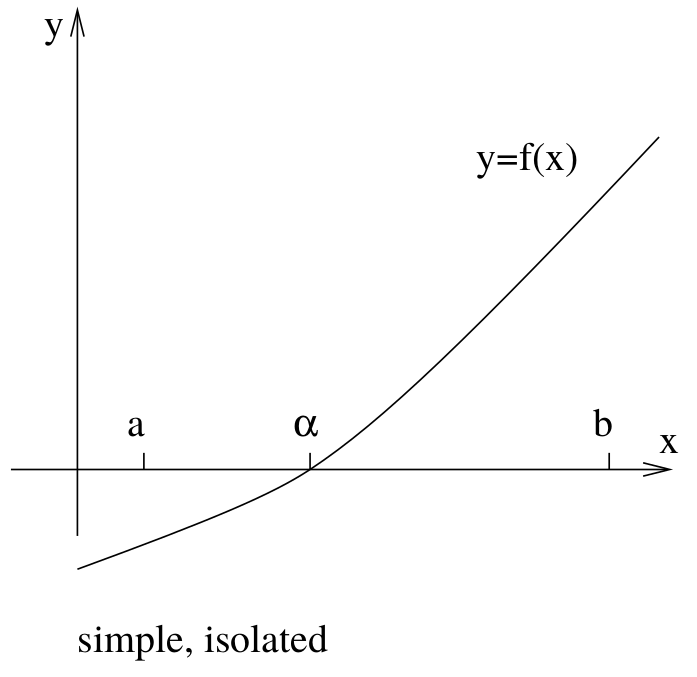
\includegraphics[width=1\linewidth]{img/7/7_1_1}
	\column{.5\linewidth}
		\centering   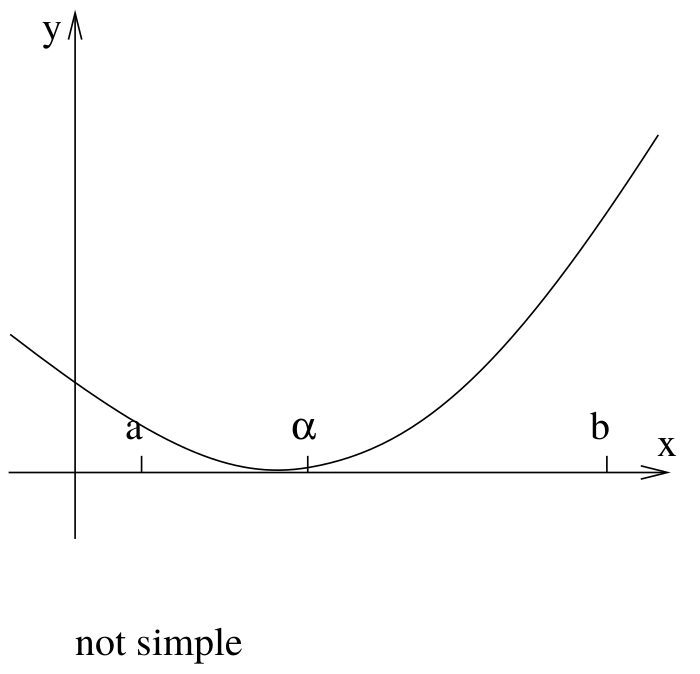
\includegraphics[width=1\linewidth]{img/7/7_1_2}
	\end{columns}
\end{frame}
%%%%%%%%%%%%%%%%
\begin{frame}{Wstęp}
	\centering 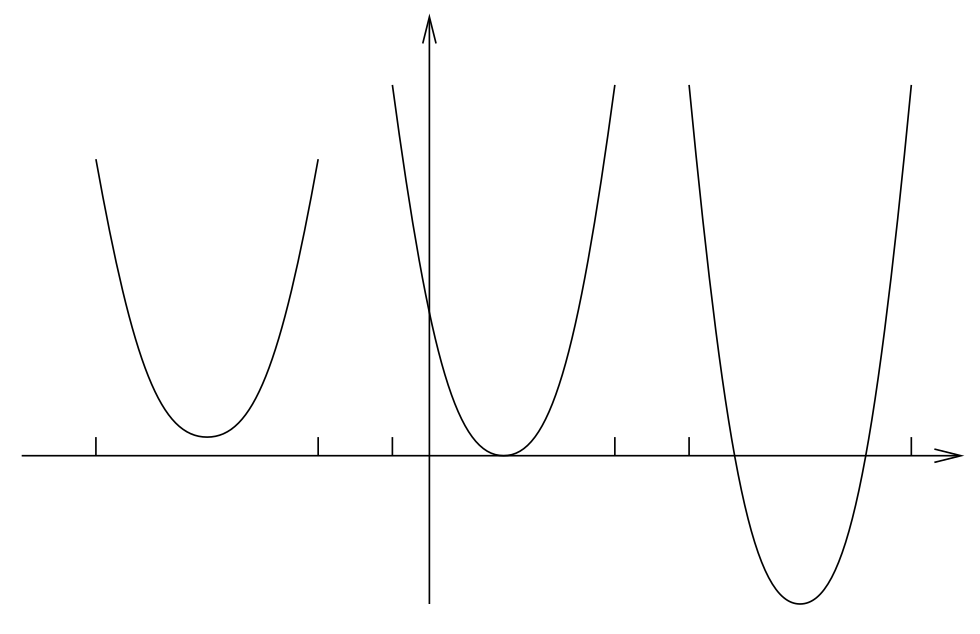
\includegraphics[width=1\linewidth]{img/7/7_1_3}
\end{frame}
%%%%%%%%%%%%%%%%
\begin{frame}{Wstęp}
	\begin{columns}
	\column{.5\linewidth}
		\centering   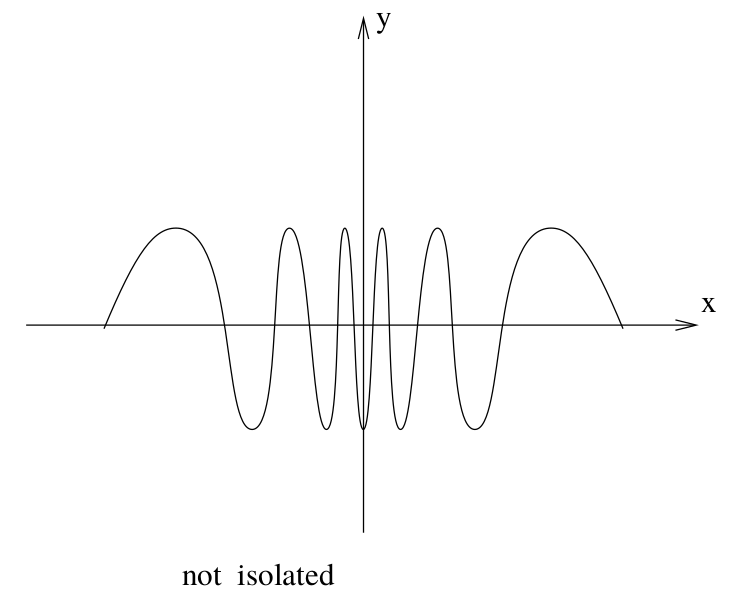
\includegraphics[width=1\linewidth]{img/7/7_1_4}
	\column{.5\linewidth}
		\centering   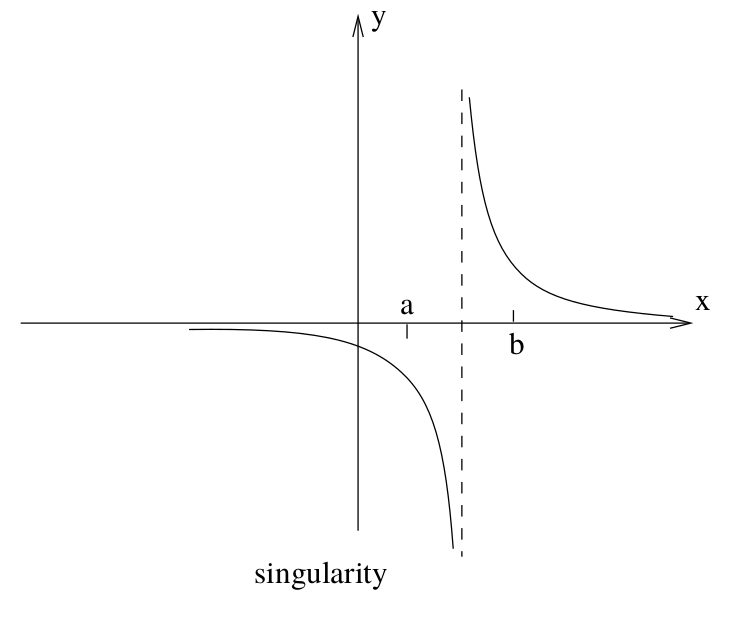
\includegraphics[width=1\linewidth]{img/7/7_1_5}
	\end{columns}
\end{frame}
%%%%%%%%%%%%%%%%
\begin{frame}{Wstęp}
	Należy więc:
	\begin{itemize}
		\item znać przebieg $f(x)$
		\item ``bracket a root''\newline
			  $\rightarrow$ przedział, w którym zmiana znaku funkcji,
		\item nie dopuszczać ``wyjść'' poza ustalony przedział.
		\item procedura szukania $\alpha$ {\bf nie może} być ``black box'' dla jej użytkownika!
	\end{itemize}
\end{frame}
%%%%%%%%%%%%%%%%
\begin{frame}{Wstęp}
	\centering   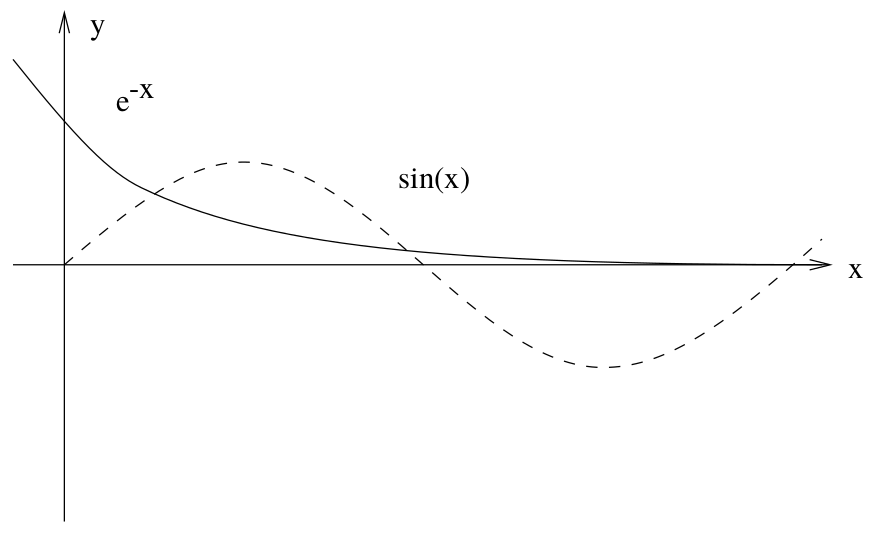
\includegraphics[width=1\linewidth]{img/7/7_1_6}
\end{frame}
	%%%%%%%%%%%%%%%%
	\section{Metoda bisekcji (połowienia)}
%%%%%%%%%%%%%%%%
\begin{frame}{Metoda bisekcji (połowienia)}
	\centering 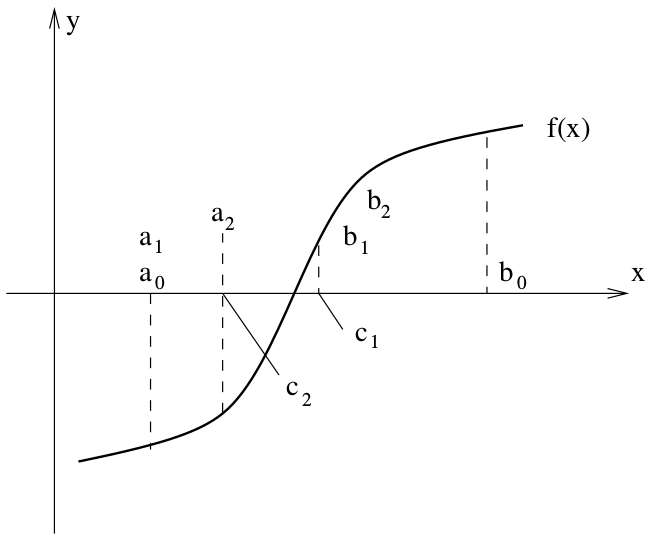
\includegraphics[width=.8\linewidth]{img/7/7_2_1}
\end{frame}
%%%%%%%%%%%%%%%%
\begin{frame}{Metoda bisekcji (połowienia)}
	\begin{table}[htbp]
		\begin{tabular}{|c|c|c|}
			\hline
			\multicolumn{1}{|c}{Dane:} & \multicolumn{2}{c|}{$a < b : \quad f(a) \cdot f(b) < 0$}\\
			\multicolumn{1}{|c}{} & \multicolumn{2}{c|}{$N$ - liczba iteracji (ustalona)}\\
			\multicolumn{1}{|c}{} & \multicolumn{2}{c|}{$d := b - a$}\\
			
			\hline
			
			\multicolumn{1}{|c}{\quad for} & \multicolumn{1}{c}{i := 1 to N do} & \text{}\\
			\cline{2-3}
			\multicolumn{1}{|c}{} & \multicolumn{2}{|c|}{c := (a + b) / 2}\\
			\cline{2-3}
			\multicolumn{1}{|c}{} & \multicolumn{2}{|c|}{f(c) $\cdot$ f(a)}\\
			\cline{2-3}
			\multicolumn{1}{|c|}{} & $<$ 0 & $>$ 0\\
			\multicolumn{1}{|c|}{} & b := c & a := c\\
			
			\hline
			
			\multicolumn{3}{|c|}{$\alpha$ := c}\\
			\multicolumn{3}{|c|}{E := d/$2^N$}\\
			\hline
		\end{tabular}
		\label{tab:transcap}
	\end{table}

	detekcja f(c) = 0\linebreak
	$\alpha$ : początkowo : w [$a_{0}$, $b_{0}$] $\rightarrow$ $b_{0}$ - $a_{0}$\linebreak
	\phantom{x} \hspace{0.2cm} po $N$ krokach : w [$a_{N}$, $b_{N}$] $\rightarrow$ błąd $\Rightarrow$
	\[
		E = b_{N} - a_{N} = \frac{b_{N-1} - a_{N-1}}{2} = \ldots = \frac{b_{0} - a_{0}}{2^{N}}
	\]
\end{frame}
%%%%%%%%%%%%%%%%
\begin{frame}{Metoda bisekcji (połowienia)}
	Charakterystyka:
	\begin{itemize}
		\item gwarancja zbieżności
		\item wolno zbieżna $\leftarrow$ wykorzystywana informacja: znak funkcji
		\item $>$ niż 1 zero $\rightarrow$ znajduje jedno z nich
		\item osobliwość $\rightarrow$ znajduje $\rightarrow$ ?
		\item kryterium zbieżności:
		\begin{itemize}
			\item $E \approx 10^{-6}$ $\rightarrow$ dobre dla $\lvert\alpha\rvert \sim 1$, złe $\rightarrow$ $\lvert\alpha\rvert \sim 10^{-26}$
			\item zwykle: $E = \epsilon \cdot \frac{a_{0} + b_{0}}{2}$ \quad $\epsilon$ - maszynowe!
			\item $\alpha \approx 0$ $\rightarrow$ specjalny przypadek
		\end{itemize}
	\end{itemize}
\end{frame}

	%%%%%%%%%%%%%%%%
	\section{Metody iteracyjne}
%%%%%%%%%%%%%%%%
\begin{frame}{Metody iteracyjne $x = \phi(x)$}
	$f(x) = 0$ zapisujemy jako \fbox{$x = \phi(x)$} - $\infty$ liczbę sposobów:\linebreak
	
	Np:\linebreak
	$x + \ln(x) = 0 \rightarrow x = -\ln(x),\quad x = e^{-x},\quad \ldots$
	$x^{3} - 3x + 1 = 0 \rightarrow x = \frac{1}{3}(x^{3} + 1), x = \frac{1}{3 - x^{2}}, x = (1 - k) \cdot x + \frac{k}{3}(x^{3} + 1)$
	
	\begin{itemize}
		\item $x_{0}$ - początkowe przybliżenie pierwiastka $\alpha$
		\item generujemy ciąg $\left\{x_{i}\right\}$ stosując proces iteracyjny:
	\end{itemize}
	\[
		x_{i} = \phi(x_{i-1}),\quad i = 1, 2, \ldots \quad lub
		\begin{cases}
			y = \phi(x_{i-1})\\
			y = x_{i}
		\end{cases}
	\]
\end{frame}
%%%%%%%%%%%%%%%%
\begin{frame}{Metody iteracyjne $x = \phi(x)$}
	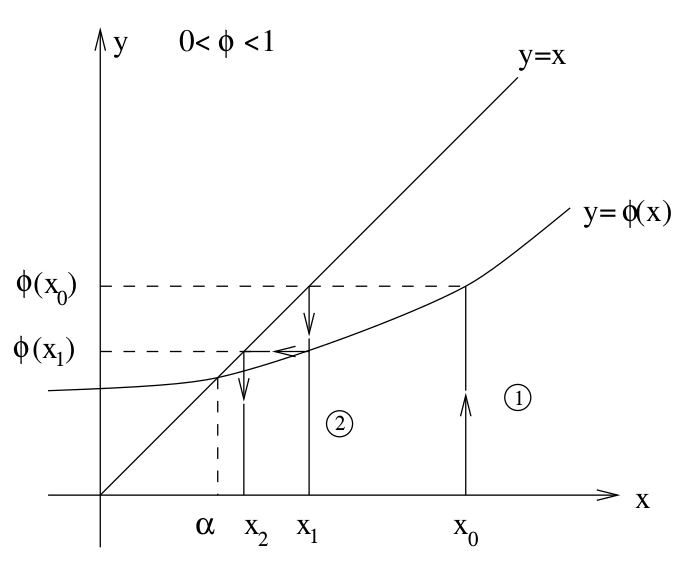
\includegraphics[width=.45\linewidth]{img/7/7_3_1}
	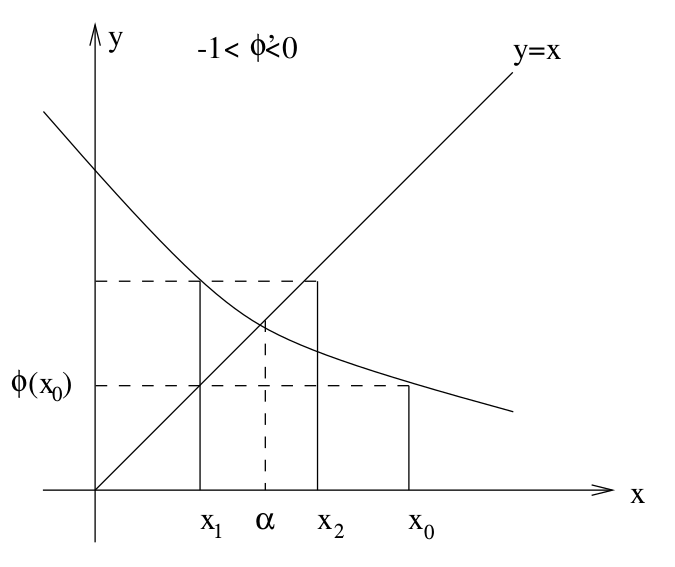
\includegraphics[width=.45\linewidth]{img/7/7_3_2}
\end{frame}
%%%%%%%%%%%%%%%%
\subsection{Twierdzenie o zbieżności procesu iteracyjnego}
\begin{frame}{Twierdzenie o zbieżności procesu iteracyjnego $x_{i+1} = \phi(x_{i})$}
	\begin{block}{Twierdzenie}
		\textbf{Niech:}
		\begin{enumerate}
			\item $x = \phi(x)$ ma pierwiastek $\alpha$
			\item na przedziale $I = \left[\alpha - a, \alpha + a\right]$ zachodzi $\lvert \phi'(x) \rvert \leq L < 1$, gdzie L jest stałą
		\end{enumerate}
		\vspace{0.5cm}
		\textbf{Wtedy: } dla dowolnego $x_{0} \in I$ :
		\begin{enumerate}
			\item $x_{i} \in I$, $i = 1, 2, \ldots$
			\item $\lim_{i \rightarrow \infty} x_{i} = \alpha$
			\item $\alpha$ jest jedynym pierwiastkiem $x = \phi(x)$ w $I$
		\end{enumerate}
	\end{block}
\end{frame}

\begin{frame}{Twierdzenie o zbieżności procesu iteracyjnego $x_{i+1} = \phi(x_{i})$}
	\textbf{Dowód:}
	\begin{enumerate}
		\item Niech $x_{i-1} \in I$
		\[
			x_{i} - \alpha = \phi(x_{i-1}) - \phi(\alpha) = (x_{i-1} - \alpha) \cdot \phi'(\eta_{i-1})
		\]
		z Tw. o wartości średniej; $\eta_{i-1} \in I$
		\[
			\lvert x_{i} - \alpha \rvert = \lvert x_{i-1} - \alpha \rvert \cdot \lvert \phi'(\eta_{i-1}) \rvert \leq \lvert x_{i-1} - \alpha \rvert \cdot L \qquad \Rightarrow x_{i} \in I \quad(*)
		\]
		
		\item $(*)$ używamy wielokrotnie
		\[
			\lvert x_{i} - \alpha \rvert \leq L \cdot \lvert x_{i-1} - \alpha \rvert \leq L^{2} \cdot \lvert x_{i-2} - \alpha \rvert \leq \ldots \leq L^{i} \cdot \lvert x_{0} - \alpha \rvert
		\]
		$L < 1$, $\lim_{i \rightarrow \infty} L^{i} = 0 \quad \Rightarrow \quad \lim_{i \rightarrow \infty} \lvert x_{i} - \alpha \rvert = 0$
	\end{enumerate}
\end{frame}
%%%%%%%%%%%%%%%
\begin{frame}{Twierdzenie o zbieżności procesu iteracyjnego $x_{i+1} = \phi(x_{i})$}
	\begin{enumerate}
		\setcounter{enumi}{2}
		\item Niech w $I$ oprócz pierwiastka $\alpha$ będzie pierwiastek $\beta$
		\[
			\alpha - \beta = \phi(\alpha) - \phi(\beta) = (\alpha - \beta) \cdot \phi'(\eta)
		\]
		\[
			\lvert \alpha - \beta \rvert = \lvert \alpha - \beta \rvert \cdot \underbrace{\lvert \phi'(\eta) \rvert}_{< 1} < \lvert \alpha - \beta \rvert \qquad \rightarrow \text{sprzeczność!}
		\]
		
		Zawsze: $x_{i-1} - \alpha = (x_{i} - \alpha) + (x_{i-1} - x_{i})$\linebreak
		Monotoniczna zbieżność\linebreak
		$\lvert x_{i-1} - \alpha \rvert \leq \lvert x_{i} - \alpha \rvert + \lvert x_{i-1} - x_{i} \rvert$ $\vert^{\cdot L + \text{fakt:}}_{\lvert x_{i} - \alpha \rvert \leq \lvert x_{i-1} - \alpha \rvert}$
		\[
			\lvert x_{i} - \alpha \rvert \leq \frac{L}{1 - L} \lvert x_{i-1} - x_{i} \rvert
		\]
		\[
			\frac{L}{1 - L} < 1 \text{ dla } L < \frac{1}{2}
		\]
	\end{enumerate}
\end{frame}
\subsection{Rząd zbieżności procedury iteracyjnej $x_{i} = \phi(x_{i-1})$}
%%%%%%%%%%%%%%
\begin{frame}{Rząd zbieżności procedury iteracyjnej $x_{i} = \phi(x_{i-1})$}
	\begin{enumerate}
		\item $\left\{x_{i}\right\} $ - zbieżność do $\alpha$
		\item ``szybkość'' zbieżności $\lvert \frac{\epsilon_{i}}{\epsilon_{i-1}} \rvert = $ ?
	\end{enumerate}
	\[
		\epsilon_{i} = x_{i} - \alpha = \phi(x_{i-1}) - \phi(\alpha)
	\]
	
	rozwinięcie względem $\alpha$
	\[
		\phi(x_{i-1}) = \sum_{j=0}^{p-1} \frac{1}{j!} \underbrace{(x_{i-1} - \alpha)^{j}}_{\epsilon_{i-1}} \cdot \phi^{(j)}(\alpha) + \frac{1}{p!}(x_{i-1}-\alpha)^{p} \cdot \phi^{(p)}(\eta_{i-1})
	\]
	
	$\eta_{i-1} \in (x_{i-1}, \alpha)$
	\[
		\epsilon_{i} = \sum_{j=1}^{p-1}\frac{1}{j!} \epsilon_{i-1}^{j} \cdot \phi^{(j)}(\alpha) + \frac{\epsilon_{i-1}^{p}}{p!} \phi^{(p)}(\eta_{i-1})
	\]
\end{frame}
%%%%%%%%%%%%%%%
\begin{frame}{Rząd zbieżności procedury iteracyjnej $x_{i} = \phi(x_{i-1})$}
	\textbf{Jeżeli: } $\phi'(\alpha) = \phi''(\alpha) = \ldots = \phi^{(p-1)}(\alpha) = 0,\quad \phi^{(p)}(\alpha) \neq 0$\linebreak
	
	\textbf{to: } $\epsilon_{i} = \frac{\epsilon_{i-1}^{p}}{p!} \phi^{(p)}(\eta_{i-1})$\linebreak
	
	$\lim_{i \rightarrow \infty} \lvert \frac{\epsilon_{i}}{\epsilon_{i-1}^{p}} \rvert = \frac{1}{p!} \lvert \phi^{(p)}(\alpha) \rvert$\linebreak
	
	$\lvert \frac{\epsilon_{i}}{\epsilon_{i-1}^{p}} \rvert$ - \textit{p-th order of convergence}\linebreak
	
	$\frac{1}{p!} \lvert \phi^{(p)}(\alpha) \rvert$ - asymptotic error constant
	\begin{tabbing}
		p = \= 1 - linear\\
		\> 2 - quadratic\\
		\> 3 - cubic
	\end{tabbing}
	
\end{frame}
%%%%%%%%%%%%%%
\begin{frame}{Rząd zbieżności procedury iteracyjnej $x_{i} = \phi(x_{i-1})$}
	Można konstruować metody iteracyjne $x_{i} = \phi(x_{i-1})$ dowolnego rzędu p - lecz: konieczne wyliczanie 0, 1, $\ldots$, $p-1$ pochodnych:\linebreak
	np. Richmod's:
	\[
	x_{i} = x_{i-1} - \frac{2 \cdot f(x_{i-1}) \cdot f'(x_{i-1})}{2 \cdot (f'(x_{i-1}))^{2} - f(x_{i-1}) f''(x_{i-1})}
	\]
\end{frame}
	%%%%%%%%%%%%%%%%
	\section{Metoda Newtona-Raphsona}
%%%%%%%%%%%%%%%%
\begin{frame}{Metoda Newtona-Raphsona}
	$f(x) = 0$, $\alpha$ - prosty pierwiastek\linebreak
	$x_{i-1}$ - przybliżenie $\alpha$\linebreak
	niech $\alpha = x_{i-1} + h$
	\[
		f(\alpha) = 0 = f(x_{i-1} + h) = f(x_{i-1}) + h \cdot f'(x_{i-1}) + \underbrace{\cdots}_{\text{pomijamy}}
	\]
	\[
		h = - \frac{f(x_{i-1})}{f'(x_{i-1})}
	\]
	\[
		\fbox{ $x_{i} = x_{i-1} - \frac{f(x_{i-1})}{f'(x_{i-1})}$ }
	\]
	\[
		\left. \begin{array}{ll}
			f(x)\\
			f'(x)
		\end{array}\right\}
	\]
\end{frame}
%%%%%%%%%%%%%%%%
\begin{frame}{Metoda Newtona-Raphsona}
	więcej informacji
	\[
		\frac{f(x_{i-1})}{h} = \tan(0) = f'(x_{i-1})
	\]
	wzór iteracyjny:
	$x = \phi(x)$, czyli $\rightarrow$ $\phi(x) = x - \frac{f(x)}{f'(x)}$\linebreak
	
	\textbf{Warunek zbieżności: } $\phi'(x) = \frac{f''(x) \cdot f(x)}{(f'(x))^{2}}$ dla $x = \alpha$ : $f'(\alpha) \neq 0$, $\phi'(\alpha) = 0$ bo $f(\alpha) = 0$\linebreak
	
	Powinno istnieć otoczenie $\alpha$, w którym $\lvert \phi'(\alpha) \rvert < 1$ tj. przy odpowiednim doborze $x_{0}$ met. N-R jest zawsze zbieżna do $\alpha$
\end{frame}
%%%%%%%%%%%%%%%%
\begin{frame}{Metoda Newtona-Raphsona}
	\centering
	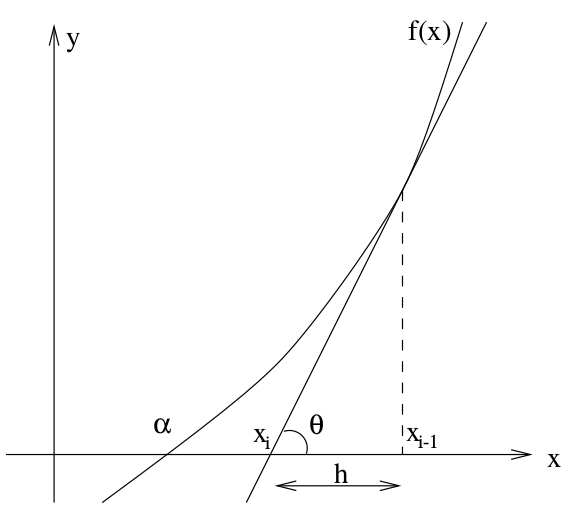
\includegraphics[width=.7\linewidth]{img/7/7_4_1}
\end{frame}
%%%%%%%%%%%%%%%%
\subsection{Twierdzenie o wyborze przedziału dla m. N-R}
\begin{frame}{Twierdzenie o wyborze przedziału dla m. N-R}
	Jeżeli: $I = \left[a, b\right]$ w którym:
	\begin{enumerate}
		\item $f(a) \cdot f(b) < 0$ - jest min. 1 pierwiastek
		\item $f'(x) \neq 0$, $x \in I$ - pierwiastek 1-krotny
		\item $f''(x) \geq 0$ lub $f''(x) \leq 0$ dla wszystkich $x \in I$\\
			(convex - wypukła) (concave = wklęsła)
		\item $\lvert \frac{f(a)}{f'(a)} \rvert < (b - a)$ i $\lvert \frac{f(b)}{f'(b)} \rvert < (b - a)$ - styczna przecinająca $x$ w $I$
	\end{enumerate}
	to:
	m. N-R jest zbieżna dla dowolnego $x_{0} \in I$ do $\alpha$
\end{frame}
%%%%%%%%%%%%%%%%
\subsection{Rząd zbieżności metody N-R}
\begin{frame}{Rząd zbieżności metody N-R}
	\begin{tabbing}
		\qquad\qquad \= $\phi(x) = x - \frac{f(x)}{f'(x)}$\\\\
		\> $\phi'(x) = \frac{f(x) \cdot f''(x)}{(f'(x))^{2}}; \quad \phi'(\alpha) = 0$\\\\
		\> $\phi''(x) = ; \quad \phi'(\alpha) \neq 0$ \quad $\clubsuit ZAD$\\
	\end{tabbing}
	- 2gi rząd tzn: $\epsilon_{i} \sim \epsilon_{i-1}^{2}$
\end{frame}
%%%%%%%%%%%%%%%%
\subsection{Dla m-krotnego pierwiastka}
\begin{frame}{Dla m-krotnego pierwiastka}
	\[
		\fbox{$x_{i} = x_{i-1} - m \cdot \frac{f(x)}{f'(x)}$}
	\]
	\linebreak
	- też o zbieżności kwadratowej \quad $\clubsuit ZAD$
\end{frame}
%%%%%%%%%%%%%%%%
\subsection{Warunek zakończenia dla m. N-R}
\begin{frame}{Warunek zakończenia dla m. N-R}
	w procedurach bibliotecznych - \textbf{rozbudowane zabezpieczenia wyznaczanie:}\linebreak\linebreak
	- $\frac{\lvert x_{i} - x_{i-1} \rvert}{\lvert x_{i} \rvert}$\linebreak\linebreak
	- $\lvert f(x_{i}) \rvert$\linebreak\linebreak
	- $\lvert f'(x_{i}) \rvert$ - zbyt mały - to może:\linebreak\linebreak
\end{frame}
%%%%%%%%%%%%%%%%
\begin{frame}{Warunek zakończenia dla m. N-R}
	\textbf{Niebezpieczeństwa:}\linebreak
	\begin{columns}
		\column{.6\linewidth}
		\centering   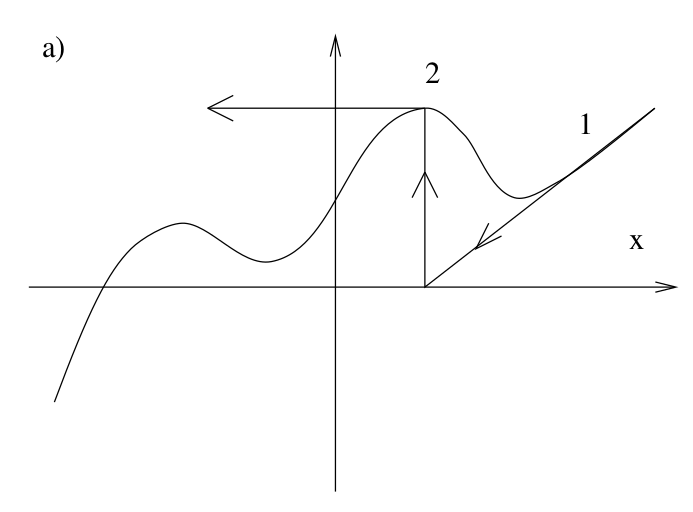
\includegraphics[width=.7\linewidth]{img/7/7_4_2}
		\column{.6\linewidth}
		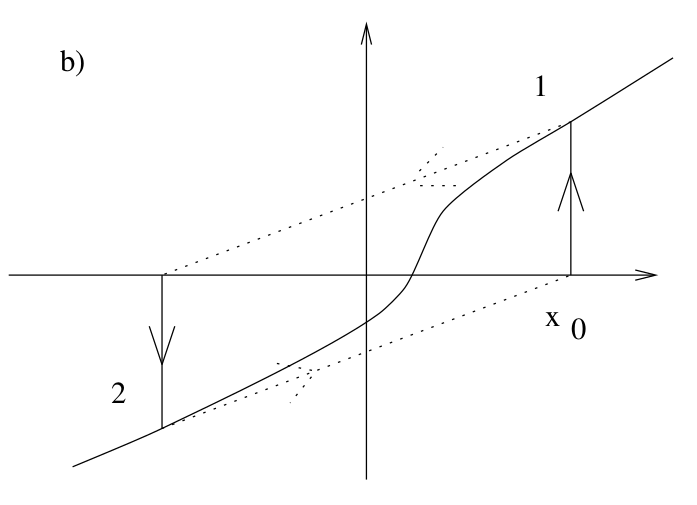
\includegraphics[width=.7\linewidth]{img/7/7_4_3}
	\end{columns}
	a) lokalne ekstrema\linebreak
	b) rozbieżny cykl iteracji możliwe, gdy f - wynik interpolacji $\Rightarrow$ inne $x_{0}$ \linebreak kombinacja: bisekcja (gdy kłopoty) + N-R
\end{frame}
	%%%%%%%%%%%%%%%%
	\section{Przyspieszanie zbieżności - metoda Aitkena}
%%%%%%%%%%%%%%%%
\begin{frame}{Przyspieszanie zbieżności - metoda Aitkena}
	$x_{i}$, $x_{i+1}$, $x_{i+2}$ - kolejne iteracje\linebreak
	\begin{tabbing}
		\quad \= $x_{i} - \alpha = \phi(x_{i-1}) - \phi(\alpha) = (x_{i-1} - \alpha) \cdot \phi'(\eta_{i-1})$, \quad $\eta_{i-1} \in (x_{i-1}, \alpha)$\\\\
		\> $x_{i+2} - \alpha = (x_{i+1} - \alpha) \cdot \phi'(\eta_{i+1})$\\\\
		\> $x_{i+1} - \alpha = (x_{i} - \alpha) \cdot \underbrace{\phi'(\eta_{i})}_{(*)}$
	\end{tabbing}
	$(*)$ - nieznane, ale w pobliżu $\alpha$; $\phi'(x) \approx$ stałe
\end{frame}
%%%%%%%%%%%%%%%%
\begin{frame}{Przyspieszanie zbieżności - metoda Aitkena}
	\[
		\frac{x_{i+2} - x_{i+2}^{*}}{x_{i+1} - x_{i+2}^{*}} = \frac{x_{i+1} - x_{i+2}^{*}}{x_{i} - x_{i+2}^{*}}
	\]
	\[
		x_{i+2}^{*} = \frac{x_{i} \cdot x_{i+2} - x_{i+1}^{2}}{x_{i+2} - 2 \cdot x_{i+1} + x_{i}} \quad \rightarrow \text{niedogodna: } L, A \rightarrow 0
	\]
	\[
		\fbox{$x_{i+2}^{*} = x_{i} - \frac{(x_{i+1} - x_{i})^{2}}{x_{i+2} - 2 \cdot x_{i+1} + x_{i}} \rightarrow (*)$}
	\]
	$(*)$ - zbieżność kwadratowa bez obliczania 2-gich pochodnych\linebreak\linebreak
	równość pochodnych \quad $\rightarrow$ \quad ze stałości:\linebreak
	\[
		\fbox{$\frac{x_{i} - x_{i-1}}{x_{i+1} - x_{i}}$}
	\]
\end{frame}
	%%%%%%%%%%%%%%%%
	\section{Metody interpolacyjne}
\subsection{Regula falsi}
\begin{frame}{Metody interpolacyjne - Regula falsi}
	\centering   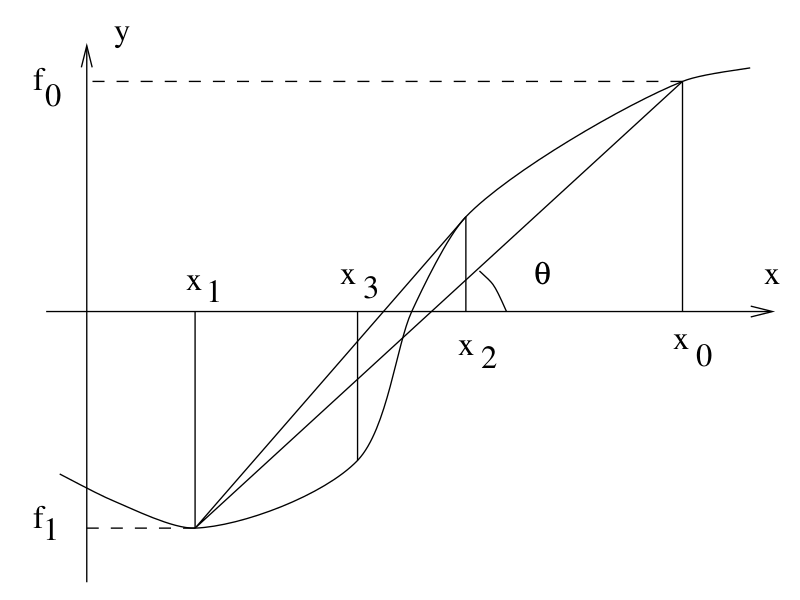
\includegraphics[width=.7\linewidth]{img/7/7_6_1}
\end{frame}
%%%%%%%%%%%%%%
\begin{frame}{Regula falsi}
	\begin{enumerate}
		\item $x_{0}$, $x_{1}$ : $f(x_{0}) \cdot f(x_{1}) < 0$
		
		\item linia prosta: $\frac{f_{0} - f_{1}}{x_{0} - x_{1}} = \frac{f_{0}}{x_{0} - x_{2}} \Rightarrow x_{2} = \frac{f_{1}}{f_{1} - f_{0}} x_{0} + \frac{f_{0}}{f_{0} - f_{1}}x_{1}$
		
		\item sprawdzenie 	$\left. \begin{array}{ll}
								f_{1} \cdot f_{2} < 0\\
								f_{0} \cdot f_{2} < 0
							\end{array}\right\} \Rightarrow x_{3} \ldots$\\
	\end{enumerate}
	- wolno zbieżna do poj. pierwiastka (zbieżność liniowa) \quad $\clubsuit ZAD$
\end{frame}
%%%%%%%%%%%%%%
\begin{frame}{Regula falsi}
	Wyjątkowo trudny przypadek:\linebreak
	\begin{center}
		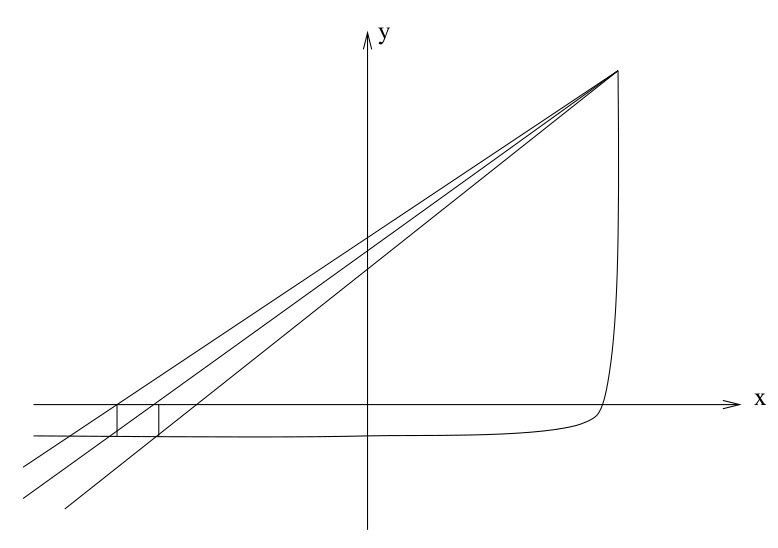
\includegraphics[width=.65\linewidth]{img/7/7_6_2}
	\end{center}
	ważne dla RF: wszystkie iteracje po tej samej stronie pierwiastka
\end{frame}
%%%%%%%%%%%%%%
\subsection{Metody Illinois i Pegasus - ulepszenie RF}
\begin{frame}{Metody Illinois i Pegasus - ulepszenie RF}
	\begin{enumerate}
		\item $x_{i}$, $x_{i+1}$, $x_{i+2}$: $\begin{cases}
			f_{i} \cdot f_{i+1} \qquad <0 $ $ \leftarrow $ obejmują pierwiastek$\\
			f_{i+1} \cdot f_{i+2} \quad <0
		\end{cases}$
		
		\item stosujemy RF do $x_{i}$, $x_{i+2}$ $\Rightarrow$ $x_{i+3}$ ale z: $f_{i} = f_{i}^{*} = \alpha \cdot f_{i}$
		
		\item gdy $f_{i+2} \cdot f_{i+3}$ $\begin{cases}
			< 0 $ - RF dla $ x_{i+2}$, $ x_{i+3}\\
			> 0 $ - zmodyf. RF dla $ x_{i}$, $x_{i+3}
		\end{cases}$
	\end{enumerate}
\end{frame}
%%%%%%%%%%%%%%
\begin{frame}{Metody Illinois i Pegasus - ulepszenie RF}
	\centering 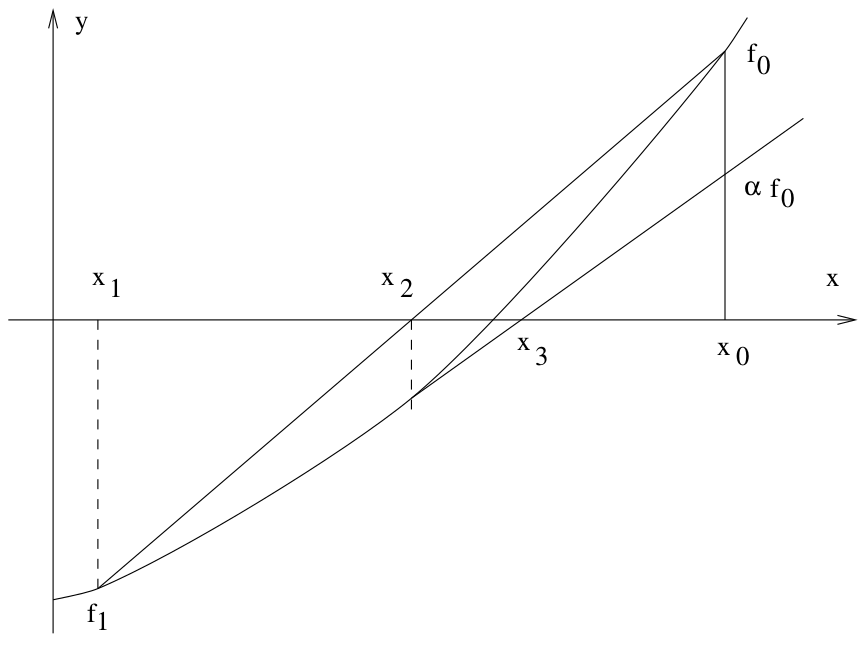
\includegraphics[width=.7\linewidth]{img/7/7_6_3} \linebreak
	\textbf{Illinois} $\rightarrow$ $\alpha = \frac{1}{2}$, \quad \textbf{Pegasus} $\rightarrow$ $\alpha = \frac{f_{0}}{f_{1} + f_{0}}$
\end{frame}
%%%%%%%%%%%%%%
\subsection{Metoda siecznych}
\begin{frame}{Metoda siecznych}
	\centering 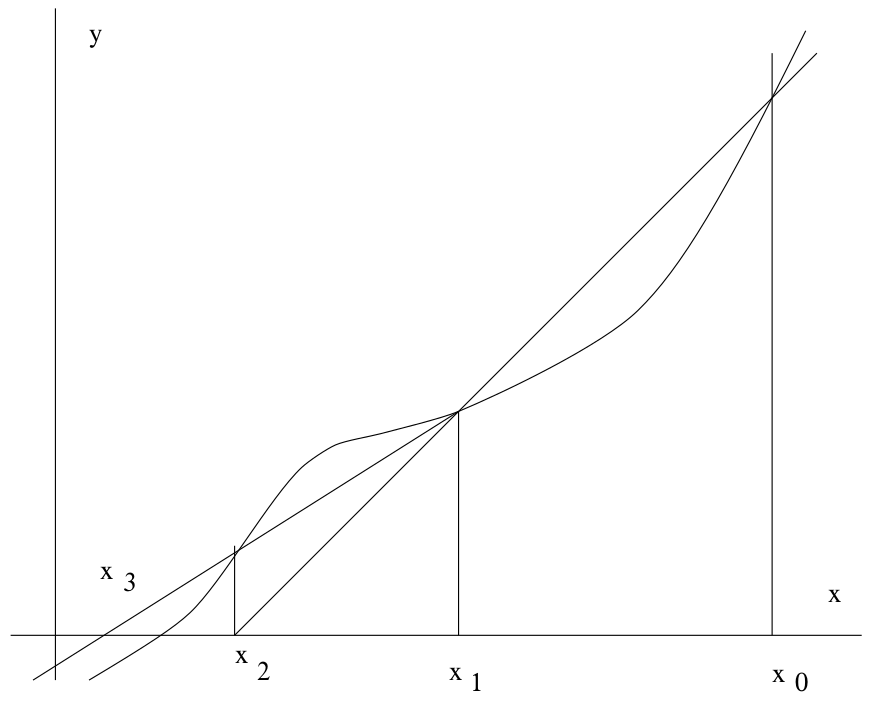
\includegraphics[width=.8\linewidth]{img/7/7_6_4}
\end{frame}
%%%%%%%%%%%%%%
\begin{frame}{Metoda siecznych}
	- $(x_{0}, x_{1})$\linebreak
	- $f_{0} \cdot f_{1}$ - nie badamy\linebreak
	linie prosta $(x_{0}, f_{0})$, $(x_{1}, f_{1})$ $\ldots$
	\[
		x_{i+2} = x_{i+1} - \underbrace{\frac{x_{i+1} - x_{i}}{f_{i+1} - f_{i}}}_{(*)} \cdot f_{i+1}
	\]
	$(*)$ - jak N-R z takim przybl. $f'(x_{i})$ \linebreak\linebreak
	- rząd zbieżności $\sim$ 1.62 \hspace{5cm} $\clubsuit ZAD$\linebreak
	- lepsza od RF\linebreak
	- gorsza od NR - lecz bez $f'$ !
\end{frame}

\end{document}
